\section{Time Windowing Experiment}

\begin{figure*}[t]
  \centerline{
    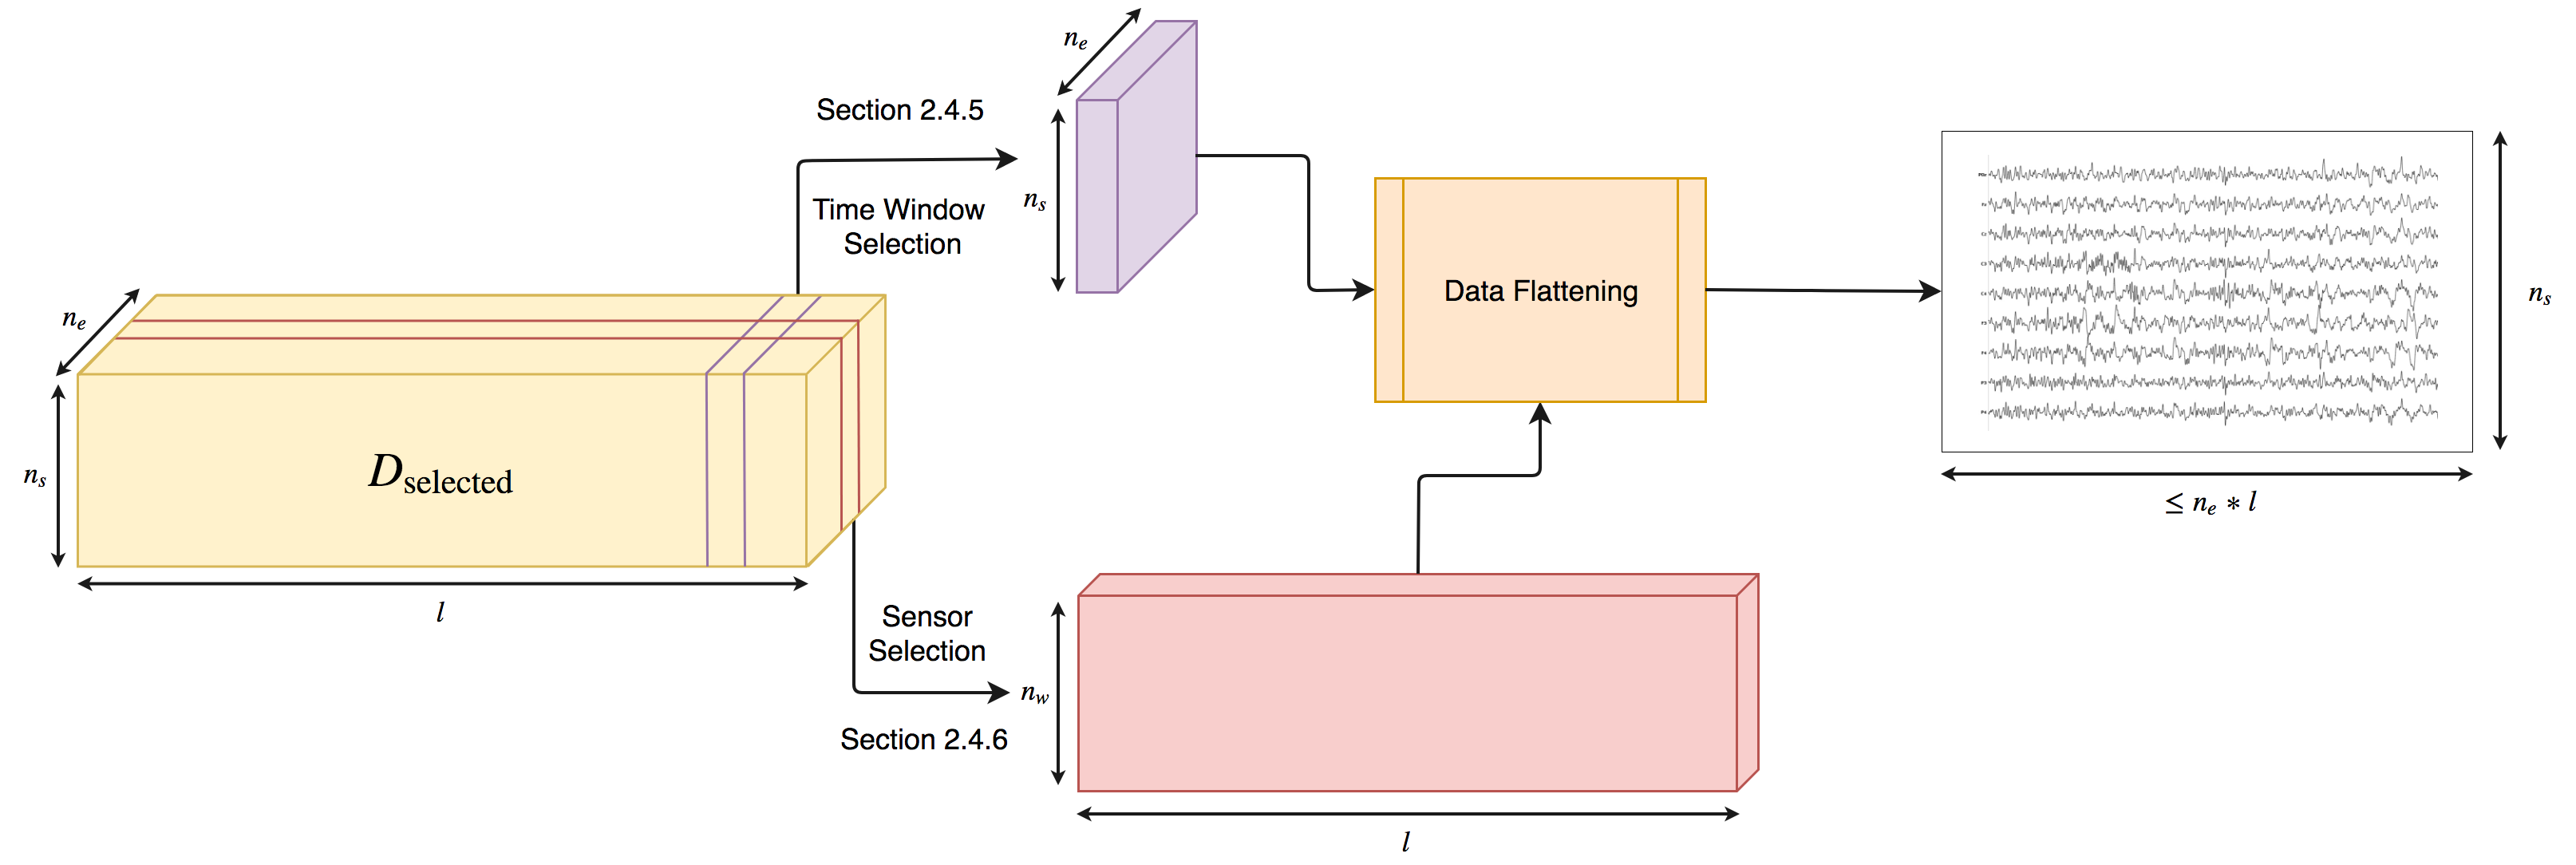
\includegraphics[width=\linewidth]{figures/reshape}
  }
  \caption[Data Reshaping Pipeline]{
    The data reshaping pipeline. Averaged trial data from $D_{\text{selected}}$ 
    can be directly passed to the reshaping process, or it can be passed 
    through another selection. We can perform two types of selection, one for 
    time analysis or one for channel analysis. We reshaped to flatten across 
    the electrode dimension, such that our training data for the model is $n_s 
    \times (n_e * l)$.
  }
  \label{fig:reshape}
\end{figure*}

We also wished to understand the recollection of a semantic representation when 
evoked by a newly learned symbol. Here, we could take advantage of EEG's high 
temporal resolution to analyze the brain's processing of symbols over time. We 
did this by separating the averaged EEG data into time windows, each 50ms long, 
and then evaluating the model pipeline on only the EEG data within a window. 
This is an additional filtering step on $D_{\text{selected}}$ that reduces the 
dimensions of $D_\text{selected}$ to $\mathbb{R}^{n_s \times (n_e * s_l)}$ 
where the length of the selected time window is defined as $s_l \leq l$. This 
process is shown in Figure~\ref{fig:reshape} as the ``Time Window Selection'' 
step. The \tvt accuracies from these groups can be visualized as a graph over 
time.

The time window with the highest accuracy represents the peak in time that the 
semantics are most strongly represented in the brain data. In their MEG 
experiments, Sudre et al.~\cite{Sudre2012} found that the decodability of nouns 
peaks in the 350ms-400ms time period after stimulus onset. We hypothesized that 
the peak accuracy for our experiment would be later, as participants must map 
each symbol to the English counterpart.
